% Document settings
\documentclass[a4paper,11pt]{article}

% Packages
  % math formulas
\usepackage{amsmath,amsthm,amssymb}
  % graphics
\usepackage{graphicx}
\usepackage{wrapfig}
  % plots
\usepackage{pgfplots}
  % other
\usepackage[warn]{mathtext}
\usepackage{cmap}
\usepackage[T1,T2A]{fontenc}
\usepackage[utf8]{inputenc}
\usepackage[english,russian]{babel}

% Package settings
%% graphicx
\graphicspath{{Pictures/}}
\DeclareGraphicsExtensions{.pdf,.png,.jpg}
%% pgfplots
\pgfplotsset{width=10cm,compat=1.9}

% Title
\title{Отчет о выполнении работы №1.2.4.}
\author{Воейко Андрей Александрович, Б01-109}
\date{Долгопрудный, 2021}

% Document
\begin{document}
\maketitle
\newpage
\section{Аннотация}
В работе измеряются периоды крутильных колебаний рамки при различных положениях закрепленного в ней тела с целью проверить теоретичесткую зависимость между периодами колебаний тела относительно нескольких осей, определить моменты инерции относительно различных осей, определить моменты инерции относительно нескольких осей для кождого тела, по ним найти главные моменты инерции.
\section{Теоретические сведения}
Тензор инерции твердого тела -- симметричная матрица, полностью определяемая шестью элементами. Из этого следует, что эту матрицу можно привести к диагональному виду. Диагональные элементы называются главными. Геометрическим образом тензора называют эллипсоид, описываемый формулой~\ref{eq1}, так называемый эллипсоид энерции.\newline
\begin{equation}    \label{eq1}
  I_{x}x^{2} + I_{y}y^{2}+ I_{z}z^{2} = 1.
\end{equation}
Координатные оси $Ox$, $Oy$, $Oz$ совпадают с главными осями тела. Если начало координат O совпадает с центром масс, то эллипсоид нызывают центральным. Сам эллипсоид же позволяет определить момент инерции относительно любой оси. Для этого проводится радиус-вектор из центра координат до пересечения с эллипсоидом вдоль этой оси. Длина r определяет момент инерции:\newline
\begin{equation}    \label{eq2}
  I = \frac{1}{r^{2}}.
\end{equation}
В данной работе используется устройство для получения крутильных колебаний, представляющее из себя рамку, закрепленную между потолком и столом двумя нитями, в которой может зажиматься груз. Крутильные колебания рамки с телом описываются уравнением~\ref{eq3}.\newline
\begin{equation}    \label{eq3}
  (I + I_{р}) \frac{d^{2}\phi}{dt^{2}} = -f\phi,
\end{equation}
Здесь $I$ -- момент инерции тела, $I_{р}$ -- момент инерции рамки, $\phi$ -- угол поворота рамки, $t$ -- время, $f$ -- модуль кручения проволоки.\newline
Пеорид определим по формуле~\ref{eq4}.\newline
\begin{equation}    \label{eq4}
  T = 2 \pi \frac{I+I_{р}}{f}
\end{equation}
Теперь предположим, что наше тело -- прямоугольный параллелепипед.\newline
\begin{wrapfigure}{r}{0.4\textwidth}
  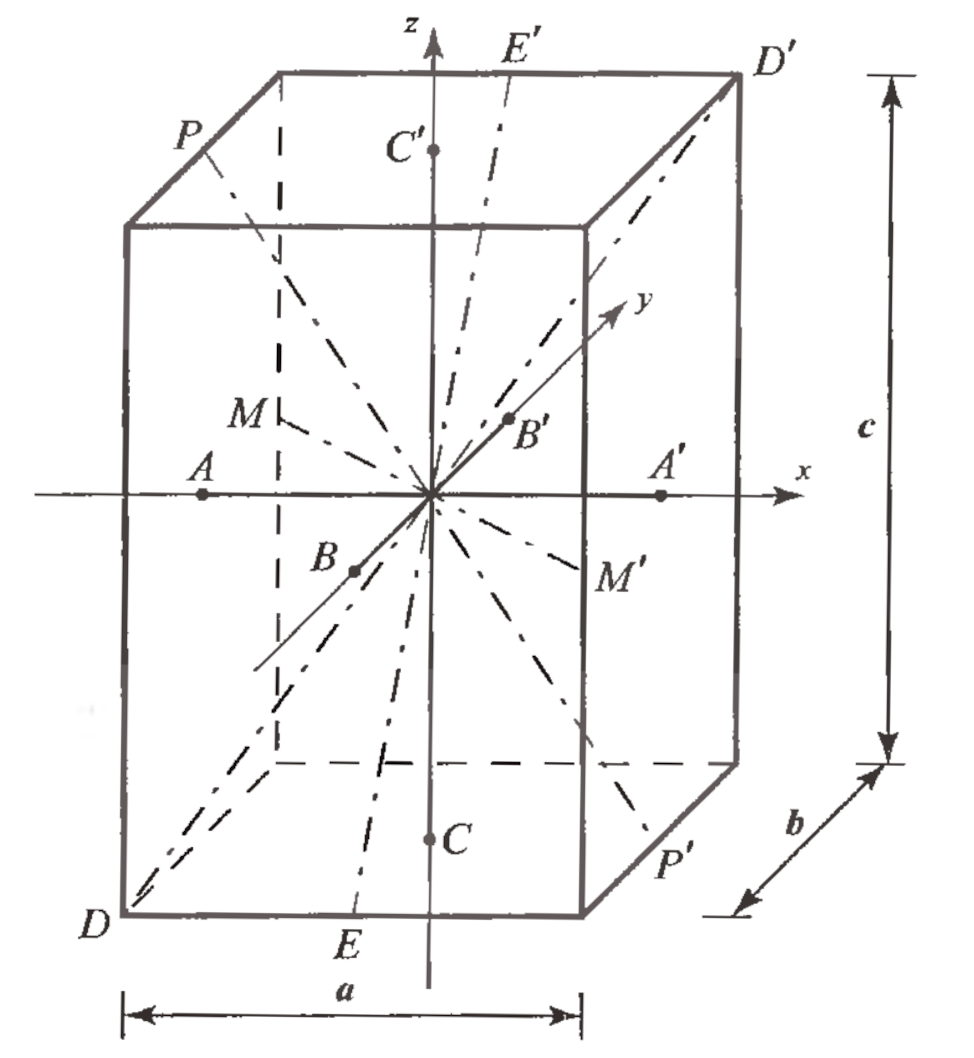
\includegraphics[scale = 0.6]{параллелепипед.png}
  \caption{Оси вращения прямоугольного параллелепипеда}
  \label{fig:img1}
\end{wrapfigure}
Согласно общей формуле~\ref{eq5},
\begin{equation}    \label{eq5}
  I = I_{x}\cos^{2}\alpha + I_{y}cos^{2}\beta + I_{z}cos^{2}\gamma,
\end{equation}
где $I$ -- момент инерции относительно произвольной оси, $\alpha$, $\beta$ и $\gamma$ -- углы между этой осью и осями $Ox$, $Oy$, $Oz$ соответственно.\newline
Рассмортрим момент инерции вдоль $DD'$. В таком случае это уравнение имеет такой вид:
\begin{equation}    \label{eq6}
I_{d} = I_{x}\frac{a^{2}}{d^{2}} + I_{y}\frac{b^{2}}{d^{2}} + I_{z}\frac{c^{2}}{d^{2}},
\end{equation}
где $I_{d}$ -- момент инерции относительно оси $DD'$, длины $a$, $b$, $c$ и $d$ -- обозначенные на рисунке $AA'$, $BB'$, $CC'$ и $DD'$ соответственно. Поскольку $d^{2} = a^{2} + b^{2} + c^{2}$, а период колебаний $T \sim \sqrt{I}$, формула~\ref{eq6} принимает вид формулы~\ref{eq7}.
\begin{equation}    \label{eq7}
  (a^{2} + b^{2} + c^{2})T_{d}^{2} = a^{2}T_{x}^{2} + b^{2}T_{y}^{2} + c^{2}T_{z}^{2}.
\end{equation}
Проверив формулу~\ref{eq7}, мы также проверим формулу~\ref{eq6}.
Аналогично, для осей $EE'$, $MM'$, $PP'$, уравнения~\ref{eq8}, \ref{eq9} и \ref{eq10} соответственно.
\begin{equation}    \label{eq8}
  (b^{2} + c^{2})T_{e}^{2} = b^{2}T_{y}^{2} + c^{2}T_{z}^{2}.
\end{equation}
\begin{equation}    \label{eq9}
  (a^{2} + c^{2})T_{e}^{2} = a^{2}T_{x}^{2} + c^{2}T_{z}^{2}.
\end{equation}
\begin{equation}    \label{eq10}
  (a^{2} + b^{2})T_{e}^{2} = a^{2}T_{x}^{2} + b^{2}T_{y}^{2}.
\end{equation}
\section{Оборудование и экспериментальная установка}
В работе используются:
\begin{itemize}
        \item Установка для получения крутильных колебаний.
        \item Исследуемые твердые тела: куб и параллелепипед.
        \item Секундомер: $\Delta_{с} = \pm 0,3\ с$ (реакция человека).
        \item Штангенциркуль: $\Delta_{шт} = \pm 0,01\ см$.
\end{itemize}
\section{Результаты измерений и обработка данных}
\subsection{Результаты измерений}
\subsubsection{Результаты измерения геомертических размеров тел} %%%%% Размеры тел %%%%%
Измерим геометрические размеры тел. Результаты представим в таблице~\ref{table:tab1}.
% Табл. 1 {{{
\begin{table}[h!]
\centering
\begin{tabular}{ ||c|c|c|c|| }
  \hline
  Тело & $a$, $см$ & $b$, $см$ & $c$, $см$ \\
  \hline
  Куб & $9,19 \pm 0,01$ & $9,20 \pm 0,01$ & $9,20 \pm 0,01$ \\
  Параллелепипед & $9,96 \pm 0,01$ & $4,95 \pm 0,01$ & $15,01 \pm 0,01$ \\
  \hline
\end{tabular}
\caption{Результаты измерений размеров тел.}
\label{table:tab1}
\end{table}
% }}}
\subsubsection{Результаты измерения периода собственных колебаний рамки} %%%%% Пустая рамка %%%%%
Измерим период собственных колебаний рамки. Результаты занесем в таблицу~\ref{table:tab2}.
% Табл. 2 {{{
\begin{table}[h!]
\centering
\begin{tabular}{ ||c|c|c|c|| }
  \hline
  № & Время & Количество & Период \\
   & колебаний $t$, $c$ & колебаний $N$ & колебаний $T_{р}$, $c$ \\
  \hline
  1 & $44,8 \pm 0,6$ & $10$ & $4,48 \pm 0,06$ \\
  2 & $45,2 \pm 0,6$ & $10$ & $4,52 \pm 0,06$ \\
  3 & $44,9 \pm 0,6$ & $10$ & $4,49 \pm 0,06$ \\
  \hline
\end{tabular}
\caption{Период колебаний пустой рамки}
\label{table:tab2}
\end{table}\newline
% }}}
Средний период колебаний составило $\overline{T_{р}} = 4,50\ с$.\newline
Стандартная ошибка среднего -- $\sigma_{\overline{T_{р}}} = 0,01\ с$.\newline
Таким образом период составил $T_{р} = 4,50 \pm 0,01\ с$.
\subsubsection{Результаты измерения периодов колебаний рамки с кубом} %%%%% Куб %%%%%
Проведем измерения периодов колебаний куба относительно всех осей. Результаты представены в таблице~\ref{table:tab3}.
% Табл. 3 {{{
\begin{table}[h!]
\centering
\begin{tabular}{ ||c|c|c|c|c|c|c|c|| }
  \hline
  Ось & $10 T_{1}$, $с$ & $T_{1}$, $с$ & $10 T_{2}$, $с$ & $T_{2}$, $с$ & $10 T_{3}$, $с$ & $T_{3}$, $с$ & $\overline{T_{к}}$ \\
  \hline
  $AA'$ & $54,2$ & $5,42$ & $53,2$ & $53,2$ & $53,6$ & $5,36$ & $5,37$ \\
   & $\pm 0,6$ & $\pm 0,06$ & $\pm 0,6$ & $\pm 0,06$ & $\pm 0,6$ & $\pm 0,06$ & $\pm 0,03$ \\
  $BB'$ & $52,9$ & $5,29$ & $53,4$ & $5,34$ & $54,3$ & $5,43$ & $5,35$ \\
   & $\pm 0,6$ & $\pm 0,06$ & $\pm 0,6$ & $\pm 0,06$ & $\pm 0,6$ & $\pm 0,06$ & $\pm 0,04$ \\
  $CC'$ & $53,8$ & $5,38$ & $53,2$ & $5,32$ & $54,1$ & $5,41$ & $5,37$ \\
   & $\pm 0,6$ & $\pm 0,06$ & $\pm 0,6$ & $\pm 0,06$ & $\pm 0,6$ & $\pm 0,06$ & $\pm 0,03$ \\
  $DD'$ & $53,6$ & $5,36$ & $53,7$ & $5,37$ & $54,0$ & $5,40$ & $5,38$ \\
   & $\pm 0,6$ & $\pm 0,06$ & $\pm 0,6$ & $\pm 0,06$ & $\pm 0,6$ & $\pm 0,06$ & $\pm 0,01$ \\
  $EE'$ & $53,5$ & $5,35$ & $54,3$ & $5,43$ & $53,2$ & $5,32$ & $5,36$ \\
   & $\pm 0,6$ & $\pm 0,06$ & $\pm 0,6$ & $\pm 0,06$ & $\pm 0,6$ & $\pm 0,06$ & $\pm 0,03$ \\
  $PP'$ & $53,2$ & $5,32$ & $54,0$ & $5,40$ & $53,6$ & $5,36$ & $5,36$ \\
   & $\pm 0,6$ & $\pm 0,06$ & $\pm 0,6$ & $\pm 0,06$ & $\pm 0,6$ & $\pm 0,06$ & $\pm 0,02$ \\
  $MM'$ & $53,2$ & $5,32$ & $53,7$ & $5,37$ & $53,4$ & $5,34$ & $5,34$ \\
   & $\pm 0,6$ & $\pm 0,06$ & $\pm 0,6$ & $\pm 0,06$ & $\pm 0,6$ & $\pm 0,06$ & $\pm 0,01$ \\
  \hline
\end{tabular}
\caption{Период колебаний рамки с кубом.}
\label{table:tab3}
\end{table}\newline
% }}}
Погрешность вычисления среднего периода колебаний вычисляется, как стандартная ошибка среднего.
\subsubsection{Результаты измерения периодов колебаний рамки с параллелепипедом} %%%%% Параллелепипед %%%%%
Проведем измерения периодов колебаний параллелепипеда относительно всех осей. Результаты представены в таблице~\ref{table:tab4}.
% Табл. 4 {{{
\begin{table}[h!]
\centering
\begin{tabular}{ ||c|c|c|c|c|c|c|c|| }
  \hline
  Ось & $10 T_{1}$, $с$ & $T_{1}$, $с$ & $10 T_{2}$, $с$ & $T_{2}$, $с$ & $10 T_{3}$, $с$ & $T_{3}$, $с$ & $\overline{T_{к}}$ \\
  \hline
  $AA'$ & $66,0$ & $6,60$ & $66,1$ & $6,61$ & $65,6$ & $6,56$ & $6,59$ \\
   & $\pm 0,6$ & $\pm 0,06$ & $\pm 0,6$ & $\pm 0,06$ & $\pm 0,6$ & $\pm 0,06$ & $\pm 0,02$ \\
  $BB'$ & $70,7$ & $7,07$ & $71,0$ & $7,10$ & $70,6$ & $7,06$ & $7,08$ \\
   & $\pm 0,6$ & $\pm 0,06$ & $\pm 0,6$ & $\pm 0,06$ & $\pm 0,6$ & $\pm 0,06$ & $\pm 0,01$ \\
  $CC'$ & $56,8$ & $5,68$ & $56,0$ & $5,60$ & $56,5$ & $5,65$ & $5,64$ \\
   & $\pm 0,6$ & $\pm 0,06$ & $\pm 0,6$ & $\pm 0,06$ & $\pm 0,6$ & $\pm 0,06$ & $\pm 0,02$ \\
  $DD'$ & $60,0$ & $6,00$ & $60,0$ & $6,00$ & $60,6$ & $6,06$ & $6,04$ \\
   & $\pm 0,6$ & $\pm 0,06$ & $\pm 0,6$ & $\pm 0,06$ & $\pm 0,6$ & $\pm 0,06$ & $\pm 0,02$ \\
  $EE'$ & $57,8$ & $5,78$ & $57,7$ & $5,77$ & $57,8$ & $5,78$ & $5,78$ \\
   & $\pm 0,6$ & $\pm 0,06$ & $\pm 0,6$ & $\pm 0,06$ & $\pm 0,6$ & $\pm 0,06$ & $\pm 0,03$ \\
  $PP'$ & $67,3$ & $6,73$ & $66,8$ & $6,68$ & $67,1$ & $6,71$ & $6,71$ \\
   & $\pm 0,6$ & $\pm 0,06$ & $\pm 0,6$ & $\pm 0,06$ & $\pm 0,6$ & $\pm 0,06$ & $\pm 0,02$ \\
  $MM'$ & $59,5$ & $5,95$ & $59,6$ & $5,96$ & $59,2$ & $5,92$ & $5,94$ \\
   & $\pm 0,6$ & $\pm 0,06$ & $\pm 0,6$ & $\pm 0,06$ & $\pm 0,6$ & $\pm 0,06$ & $\pm 0,01$ \\
  \hline
\end{tabular}
\caption{Период колебаний рамки с параллелепипедом.}
\label{table:tab4}
\end{table}\newline
% }}}
Погрешность вычисления среднего периода колебаний вычисляется, как стандартная ошибка среднего.
\subsection{Обработка данных}
\subsubsection{Сечения эллипсоидов инерции главными плоскостями}
Построим сечения эллипсоидов инерции с основными плоскостями. Для этого необходимо вычислить величину $\frac{10}{\sqrt{T^{2} - T_{р}^{2}}}$ для каждой из осей. Результаты представлены в таблице~\ref{table:tab5} для куба и таблице~\ref{table:tab6} для параллелепипеда.
% Табл. 5 {{{
\begin{table}[h!]
\centering
\begin{tabular}{ ||c|c|| }
  \hline
  Ось & Величина $\frac{10}{\sqrt{T^{2} - T_{р}^{2}}}$, $c^{-1}$ \\
  \hline
  $x\ (AA')$ & $2,0 \pm 0,1$ \\
  $y\ (BB')$ & $2,0 \pm 0,1$ \\
  $z\ (CC')$ & $2,0 \pm 0,1$ \\
  $x\ +\ y\ (MM')$ & $2,0 \pm 0,1$ \\
  $y\ +\ y\ (EE')$ & $2,0 \pm 0,1$ \\
  $x\ +\ z\ (PP')$ & $2,0 \pm 0,1$ \\
  \hline
\end{tabular}
    \caption{Величина $\frac{10}{\sqrt{T^{2} - T_{р}^{2}}}$ для осей, находящихся в главных плоскотях для куба.}
\label{table:tab5}
\end{table}\newline
% }}}
% Табл. 6 {{{
\begin{table}[h!]
\centering
\begin{tabular}{ ||c|c|| }
  \hline
  Ось & Величина $\frac{10}{\sqrt{T^{2} - T_{р}^{2}}}$, $c^{-1}$ \\
  \hline
  $x\ (AA')$ & $1,6 \pm 0,1$ \\
  $y\ (BB')$ & $1,5 \pm 0,1$ \\
  $z\ (CC')$ & $1,9 \pm 0,1$ \\
  $x\ +\ y\ (MM')$ & $1,6 \pm 0,1$ \\
  $y\ +\ y\ (EE')$ & $1,9 \pm 0,1$ \\
  $x\ +\ z\ (PP')$ & $1,8 \pm 0,1$ \\
  \hline
\end{tabular}
    \caption{Величина $\frac{10}{\sqrt{T^{2} - T_{р}^{2}}}$ для осей, находящихся в главных плоскотях для параллелепипеда.}
\label{table:tab6}
\end{table}\newline
% }}}
% Граф. 1 {{{
\begin{center}
\begin{tikzpicture}
\begin{axis}[
	xlabel = {$x$},
	ylabel = {$y$},
    xmin = -3,
    xmax = 3,
    ymin = -2.5,
    ymax = 2.5,
    grid = major,
	minor tick num = 6
]
\addplot[
    mark size=2pt,
    only marks,
    blue,
]
table {
	x     y
	2     0
	1.41  1.41
	0     2
	-1.41 1.41
    -2    0
    -1.41 -1.41
    0     -2
    1.41  -1.41
};
\addplot[blue, samples = 300] { sqrt(4 - x^2) };
\addplot[blue, samples = 300] { -sqrt(4 - x^2) };
\end{axis}
\end{tikzpicture}\newline
Рисунок 1: Сечение эллипсоида инерции куба плоскостью $x$, $y$.\newline
\end{center}
% }}}
% Граф. 2 {{{
\begin{center}
\begin{tikzpicture}
\begin{axis}[
	xlabel = {$y$},
	ylabel = {$z$},
    xmin = -3,
    xmax = 3,
    ymin = -2.5,
    ymax = 2.5,
    grid = major,
	minor tick num = 6
]
\addplot[
    mark size=2pt,
    only marks,
    red,
]
table {
	x     y
	2     0
	1.41  1.41
	0     2
	-1.41 1.41
    -2    0
    -1.41 -1.41
    0     -2
    1.41  -1.41
};
\addplot[red, samples = 300] { sqrt(4 - x^2) };
\addplot[red, samples = 300] { -sqrt(4 - x^2) };
\end{axis}
\end{tikzpicture}\newline
Рисунок 2: Сечение эллипсоида инерции куба плоскостью $y$, $z$.\newline
\end{center}
% }}}
% Граф. 3 {{{
\begin{center}
\begin{tikzpicture}
\begin{axis}[
	xlabel = {$x$},
	ylabel = {$z$},
    xmin = -3,
    xmax = 3,
    ymin = -2.5,
    ymax = 2.5,
    grid = major,
	minor tick num = 6
]
\addplot[
    mark size=2pt,
    only marks,
    green,
]
table {
	x     y
	2     0
	1.41  1.41
	0     2
	-1.41 1.41
    -2    0
    -1.41 -1.41
    0     -2
    1.41  -1.41
};
\addplot[green, samples = 300] { sqrt(4 - x^2) };
\addplot[green, samples = 300] { -sqrt(4 - x^2) };
\end{axis}
\end{tikzpicture}\newline
Рисунок 3: Сечение эллипсоида инерции куба плоскостью $x$, $z$.\newline
\end{center}
% }}}
% Граф. 4 {{{
\begin{center}
\begin{tikzpicture}
\begin{axis}[
	xlabel = {$x$},
	ylabel = {$y$},
    xmin = -3,
    xmax = 3,
    ymin = -2.5,
    ymax = 2.5,
    grid = major,
	minor tick num = 6
]
\addplot[
    mark size=2pt,
    only marks,
    blue,
]
table {
	x     y
    1.6   0
	1.3   0.9
	0     1.5
	-1.3  0.9
    -1.6  0
    -1.3  -0.9
    0     -1.5
    1.3   -0.9
};
\addplot[blue, samples = 300] {  0.9375*sqrt(2.56 - x^2) };
\addplot[blue, samples = 300] { -0.9375*sqrt(2.56 - x^2) };
\end{axis}
\end{tikzpicture}\newline
Рисунок 4: Сечение эллипсоида инерции параллелепипеда плоскостью $x$, $y$.\newline
\end{center}
% }}}
% Граф. 5 {{{
\begin{center}
\begin{tikzpicture}
\begin{axis}[
	xlabel = {$y$},
	ylabel = {$z$},
    xmin = -3,
    xmax = 3,
    ymin = -2.5,
    ymax = 2.5,
    grid = major,
	minor tick num = 6
]
\addplot[
    mark size=2pt,
    only marks,
    red,
]
table {
	x     y
	1.5   0
	0.81  1.62
	0     1.9
	-0.81 1.62
    -1.5  0
    -0.81 -1.62
    0     -1.9
    0.81  -1.62
};
\addplot[red, samples = 300] {  1.2667*sqrt(2.25 - x^2) };
\addplot[red, samples = 300] { -1.2667*sqrt(2.25 - x^2) };
\end{axis}
\end{tikzpicture}\newline
Рисунок 5: Сечение эллипсоида инерции параллелепипеда плоскостью $y$, $z$.\newline
\end{center}
% }}}
% Граф. 6 {{{
\begin{center}
\begin{tikzpicture}
\begin{axis}[
	xlabel = {$x$},
	ylabel = {$z$},
    xmin = -3,
    xmax = 3,
    ymin = -2.5,
    ymax = 2.5,
    grid = major,
	minor tick num = 6
]
\addplot[
    mark size=2pt,
    only marks,
    green,
]
table {
	x     y
	1.6   0
	1.05  1.47
	0     1.9
	-1.05 1.47
    -1.6  0
    -1.05 -1.47
    0     -1.9
    1.05  -1.47
};
\addplot[green, samples = 300] {  1.1875*sqrt(2.56 - x^2) };
\addplot[green, samples = 300] { -1.1875*sqrt(2.56 - x^2) };
\end{axis}
\end{tikzpicture}\newline
Рисунок 6: Сечение эллипсоида инерции параллелепипеда плоскостью $x$, $z$.\newline
\end{center}
% }}}
\subsubsection{Проверка справедливости формул~\ref{eq7}--\ref{eq10}}
Проверим справедливость формул~\ref{eq7}--\ref{eq10}.\newline
$(a^{2} + b^{2} + c^{2}) (T_{d}^{2} - T_{р}^{2}) = 5730 \pm 90$.\newline\newline
$a^{2}(T_{x}^{2} - T_{р}^{2}) + b^{2}(T_{y}^{2} - T_{р}^{2}) + c^{2}(T_{z}^{2} - T_{р}^{2}) = 5700 \pm 90$.\newline\newline
$(b^{2} + c^{2}) (T_{e}^{2} - T_{р}^{2}) = 3330 \pm 50$.\newline\newline
$b^{2}(T_{y}^{2} - T_{р}^{2}) + c^{2}(T_{z}^{2} - T_{р}^{2}) = 3380 \pm 60$.\newline\newline
$(a^{2} + c^{2}) (T_{p}^{2} - T_{р}^{2}) = 4940 \pm 70$.\newline\newline
$a^{2}(T_{x}^{2} - T_{р}^{2}) + c^{2}(T_{z}^{2} - T_{р}^{2}) = 4960 \pm 80$.\newline\newline
$(a^{2} + b^{2}) (T_{m}^{2} - T_{р}^{2}) = 3080 \pm 30$.\newline\newline
$a^{2}(T_{x}^{2} - T_{р}^{2}) + b^{2}(T_{y}^{2} - T_{р}^{2}) = 3050 \pm 30$.\newline\newline
\section{Выводы}
В ходе работы были найдены периоды колебаний двух тел в различных осях. Были построены проекции эллипсов инерции в основных плоскостях. Была проверена справедливость формул~\ref{eq7}--\ref{eq10}. Полученные значения лежат в пределах погрешности.
\end{document}
